\subsection{Funktionsweise}
\label{subsec:cdfunktionsweise}

Die Compact Disc besteht aus einer Polycarbonatscheibe und einer 40-80 nm
dicken. zumeist aus Aluminium bestehenden Reflexionsschicht. Zusätzlich gibt es
noch eine 10-20 µm dicke Lackschicht, welche die Reflexionsschicht schützt.
Zusammen genommen ergibt dies eine Höhe von ca. 1,2 mm (siehe
\autoref{fig:cdquer}). Außerdem lässt sich eine Einbuchtung (\textit{pit})
erkennen, die sich von der Grundebene (\textit{land}) abhebt. \cite{cfcd}

\begin{figure}[h]
    \begin{center}
        \begin{minipage}[t]{\textwidth}
            \begin{center}
                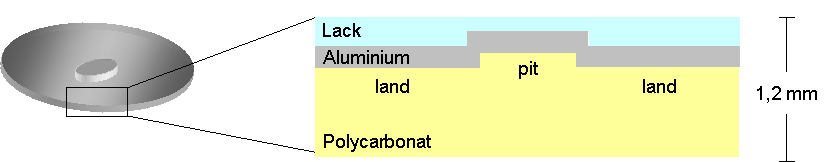
\includegraphics[height=0.1\textheight]{Bilder/Optische_Datentraeger_Die_Compact_Disc/Funktionsweise/cdquer.png}
                \caption[Querschnitt einer CD (Skizze) \newline \url{http://daten.didaktikchemie.uni-bayreuth.de/umat/cd_dvd/cd_dvd.htm} (zuletzt aufgerufen am 07.08.2015)]{Querschnitt einer CD (Skizze)}
                \label{fig:cdquer}
            \end{center}
        \end{minipage}
    \end{center}
\end{figure}

Die Abtasteinheit, bestehend aus einem Laser und einem Fotodetektor, liest
spiralförmig von innen nach außen die Informationen auf der CD aus. Dafür
wandelt der Fotodetektor das Laserlicht, das durch die Polycarbonatscheibe geht
und von der Reflexionsschicht zurückgeworfene wird, in Strom um, wobei die
Stromstärke abhängig von der Lichtintensität ist. Überstreift der
Laserstrahl ein \textit{pit}, nehmen Lichtintensität und damit auch die
Stromstärke ab. Da der Durchmesser des Laserstrahls größer als die Pitbreite
ist (siehe \autoref{fig:cdrem}), trifft dieser nur teilweise auf den
\textit{pit}. Der Rest des Lichtes trifft etwas früher auf den umgebenden
\textit{land}. Die Verschiebung der Strahlen gegeneinander, welche man in
\autoref{fig:cdlaser} erkennen kann, resultiert in einer Intensitätsabnahme, da
es aufgrund der destruktiven Interferenz\footnote{Wellenberg und Wellental
zweier Lichtstrahlen mit gleicher Frequenz und Amplitude treffen aufeinander und
heben sich gegenseitig auf.} zu einer teilweisen Auslöschung des Laserlichts
kommt. \autoref{fig:cdstrom} zeigt einen möglichen Stromstärkenverlauf. Den
Übergänge zwischen \textit{pit} und \textit{land} wird der Binärwert 1
zugewiesen. Dies entspricht dem Schnittpunkt zwischen dem Mittelwert und dem
Graph der Stromstärke in \autoref{fig:cdstrom}. \cite{cdp}

\begin{figure}[h]
    \begin{center}
        \begin{minipage}[t]{0.3\textwidth}
            \begin{center}
                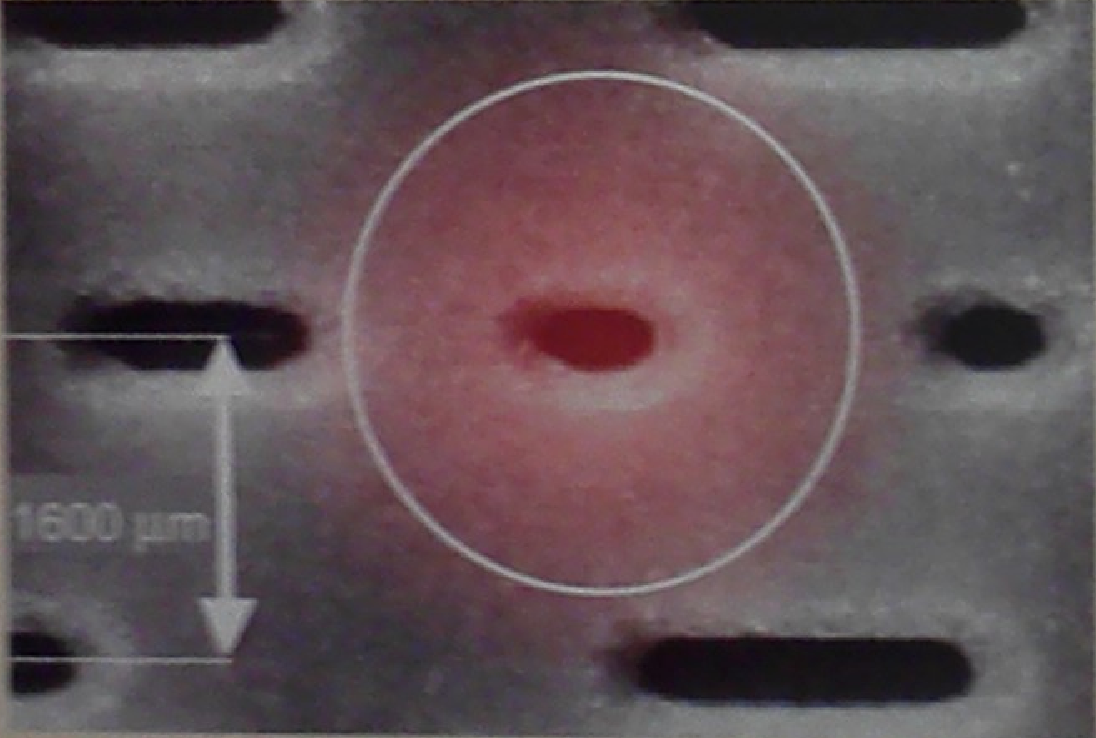
\includegraphics[height=0.1\textheight]{Bilder/Optische_Datentraeger_Die_Compact_Disc/Funktionsweise/remcd.png}
                \caption[Laserlicht auf einem \textit{pit} unter einem Rasterelektronenmikroskop \newline Roth, Klaus: CD, DVD \& Co.: Die Chemie der schillernden Scheiben, in: Chemie in unserer Zeit (41/2007), S. 340]{Laserlicht auf einem \textit{pit} unter einem Rasterelektronenmikroskop}
                \label{fig:cdrem}
            \end{center}
        \end{minipage}
        \hspace{0.025\textwidth}
        \begin{minipage}[t]{0.3\textwidth}
            \begin{center}
                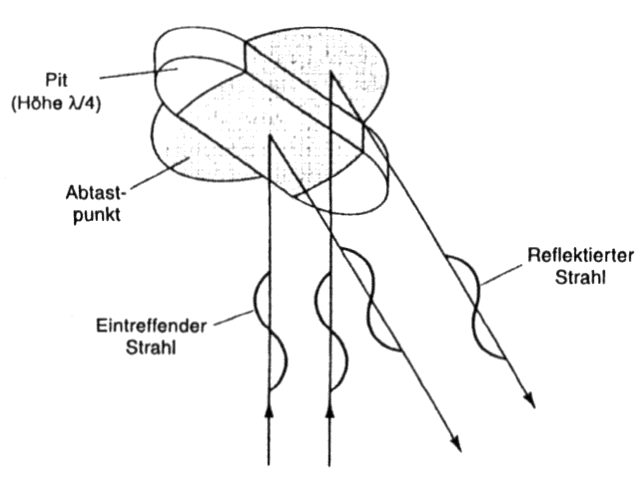
\includegraphics[height=0.1\textheight]{Bilder/Optische_Datentraeger_Die_Compact_Disc/Funktionsweise/cdlaser.png}
                \caption[destruktive Interferenz von Laserlicht bei einem \textit{pit} (Skizze) \newline \url{http://www.muenster.de/~asshoff/physik/cd/image50.gif} (zuletzt aufgerufen am 07.08.2015)]{destruktive Interferenz von Laserlicht bei einem \textit{pit} (Skizze)}
                \label{fig:cdlaser}
            \end{center}
        \end{minipage}
        \hspace{0.025\textwidth}
        \begin{minipage}[t]{0.3\textwidth}
            \begin{center}
                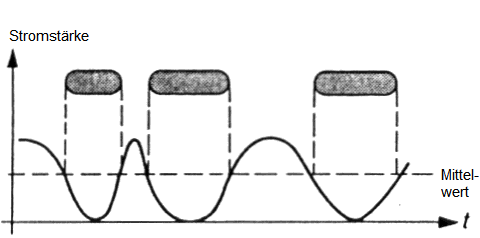
\includegraphics[height=0.09\textheight]{Bilder/Optische_Datentraeger_Die_Compact_Disc/Funktionsweise/cdstrom.png}
                \caption[Stromstärkenverlauf \newline \url{http://www.muenster.de/~asshoff/physik/cd/image51.gif} (zuletzt aufgerufen am 07.08.2015)]{Stromstärkenver-lauf}
                \label{fig:cdstrom}
            \end{center}
        \end{minipage}
    \end{center}
\end{figure}

%TODO: Referenz auf Material: Polycarbonat?
